\documentclass[letterpaper, 12pt]{article}
% \usepackage{fontspec}

% ==================================================

% document parameters
\usepackage[english]{babel}
\usepackage[margin = 1in]{geometry}

% ==================================================

% Packages for math
%\usepackage{mathrsfs}
%\usepackage{amsfonts}
%\usepackage{amsmath}
%\usepackage{amsthm}
%\usepackage{amssymb}
%\usepackage{physics}
%\usepackage{dsfont}
%\usepackage{esint}

% ==================================================

% Packages for writing
%\usepackage{enumerate}
\usepackage[shortlabels]{enumitem}
\usepackage{framed}
\usepackage{csquotes}

% ==================================================

% Miscellaneous packages
\usepackage{float}
\usepackage{tabularx}
\usepackage{xcolor}
\usepackage{multicol}
\usepackage{subcaption}
\usepackage{caption}
\captionsetup{format = hang, margin = 10pt, font = small, labelfont = bf}

% Citation
\usepackage[round, authoryear]{natbib}

% Hyperlinks setup
\usepackage{hyperref}
\definecolor{links}{rgb}{0.36,0.54,0.66}
\hypersetup{
   colorlinks = true,
    linkcolor = black,
     urlcolor = blue,
    citecolor = blue,
    filecolor = blue,
    pdfauthor = {Author},
     pdftitle = {Title},
   pdfsubject = {subject},
  pdfkeywords = {one, two},
  pdfproducer = {LaTeX},
   pdfcreator = {pdfLaTeX},
   }
   
% enable better typesetting
\usepackage{microtype}

\usepackage[T1]{fontenc}
\usepackage{inconsolata}

\usepackage{color}

\definecolor{pblue}{rgb}{0.13,0.13,1}
\definecolor{pgreen}{rgb}{0,0.5,0}
\definecolor{pred}{rgb}{0.9,0,0}
\definecolor{pgrey}{rgb}{0.46,0.45,0.48}

\usepackage{listings}


\usepackage{listings}
\lstset{
	language=Python,
	frame=none,
	firstnumber=last,
	escapeinside={(*@}{@*)},
	breaklines=false,
	breakatwhitespace=true,
	commentstyle=\color{pgreen},
	keywordstyle=\color{pblue},
	stringstyle=\color{pred},
	basicstyle=\ttfamily\footnotesize,
	moredelim=[il][\textcolor{pgrey}]{$$},
	moredelim=[is][\textcolor{pgrey}]{\%\%}{\%\%},
	xleftmargin=.125in,
	tabsize=4,
	keepspaces=true,
	emph={@staticmethod,@classmethod,@property},
	emphstyle=\color{purple}\bfseries,
}


\usepackage{here}
\usepackage{textgreek}
\usepackage{enumitem}
\usepackage{textcase}
\usepackage{titlesec}
\usepackage[many]{tcolorbox}

% Adjust spacing after the chapter title
\titlespacing*{\chapter}{0cm}{-2.0cm}{0.50cm}
\titlespacing*{\section}{0cm}{0.50cm}{0.25cm}

% Indent 
\setlength{\parindent}{0pt}
\setlength{\parskip}{1ex}

% --- Theorems, lemma, corollary, postulate, definition ---
% \numberwithin{equation}{section}

\newtcbtheorem[]{example_}{Example}%
    {enhanced,
    colback = black!5, %white,
    colbacktitle = black!5,
    coltitle = black,
    boxrule = 0pt,
    frame hidden,
    borderline west = {0.5mm}{0.0mm}{black},
    fonttitle = \bfseries\sffamily,
    breakable,
    before skip = 3ex,
    after skip = 3ex,
	label={example:\thetcbcounter},
}{example_}


\newenvironment{example}[2][] % optional title
{
\begin{example_}{#1}{}
#2
}
{
\end{example_}
}



\tcbuselibrary{skins, breakable}

% --- You can define your own color box. Just copy the previous \newtcbtheorm definition and use the colors of yout liking and the title you want to use.
\newcommand{\keyword}[1]{\textsc{\MakeTextLowercase{\smallcapsfont #1}}}
\renewcommand{\thesection}{\Roman{section}.} 
\renewcommand{\thesubsection}{\alph{subsection})}
\renewcommand{\thesubsubsection}{\arabic{subsubsection}.}
\usepackage{fontspec}

% Main font family: Baskerville 1757
\setmainfont[
Path = fonts/,
UprightFont = Baskerville1757.ttf,
ItalicFont = baskerville-1757-italic.ttf,
BoldFont = Baskerville-10-Pro-Bold_6068.ttf,
BoldItalicFont = Baskerville-10-Pro-Bold-Italic_6067.ttf,
Ligatures = TeX,
SmallCapsFont={lmromancaps10-regular.otf},
SmallCapsFeatures={Letters=SmallCaps}
]{Baskerville1757.ttf}

% Monospaced font: Inconsolata
\setmonofont[
Path = fonts/,
AutoFakeSlant,
Scale = MatchLowercase
]{Inconsolata.otf}


% Small caps font: LM Roman Caps with FakeBold
\newfontfamily\smallcapsfont[
Path = fonts/,
Letters = SmallCaps,
FakeBold = 0.05  % Slightly thicker small caps
]{lmromancaps10-regular.otf}


\begin{document}

\begin{Large}
    \textsf{\textbf{Term Project Proposal}}
    
    Tabletop Role Playing Game Information Manager
\end{Large}

\vspace{1ex}

\text{Richard Broderick}



\section{Problem statement}
In the course of running a Tabletop Role Playing Game(\keyword{TTRPG}) the creation, managing and updating of various pieces of information is one of the primary tasks of the Game Master(\keyword{GM}). In particular the cast of characters that the players interact with called \keyword{NPCs}. Having a tool that can present this data and allow its quick lookup would make the seamless running of the game and story more easily possible.
\section{Description of users/audience}
This tool would be mostly helpful for those who want to run a \keyword{TTRPG} game. Typically this person is called the Game Master who will use the program to record and create new \keyword{NPCs}. Adding the use of local \keyword{LLMs} allows for giving name and image creation suggestions. 

Another audience could be used for those who need to manage characters such as writers, they could use it as a tool to map characters in a story and hold notes about them.
\section{Core features}
\begin{description}
	\item [$\bullet$ -- C] The ability to create new \keyword{NPCs}.
	\begin{itemize}
		\item Connection to local \keyword{LLM} via llamafile to generate data suggestions, such as names
		\item Ability to add images such as profile image, 
		\begin{itemize}
			\item Giving the ability to generate with local \keyword{LLM} Stable Diffusion.
		\end{itemize}
	\end{itemize}
	\item [$\bullet$ -- R] Search existing \keyword{NPCs} read the data and find via various fields such as name or faction.
	\item [$\bullet$ -- U] Update \keyword{NPC} information as needed.
	\item [$\bullet$ -- D] Delete \keyword{NPCs} from the database.
	\item [$\bullet$] Utilize python and the customtkinter \keyword{GUI} library to create a desktop application.
\end{description}
\section{Preliminary ERD}

\begin{figure}[H]
	\caption{ERD}
	\centering
	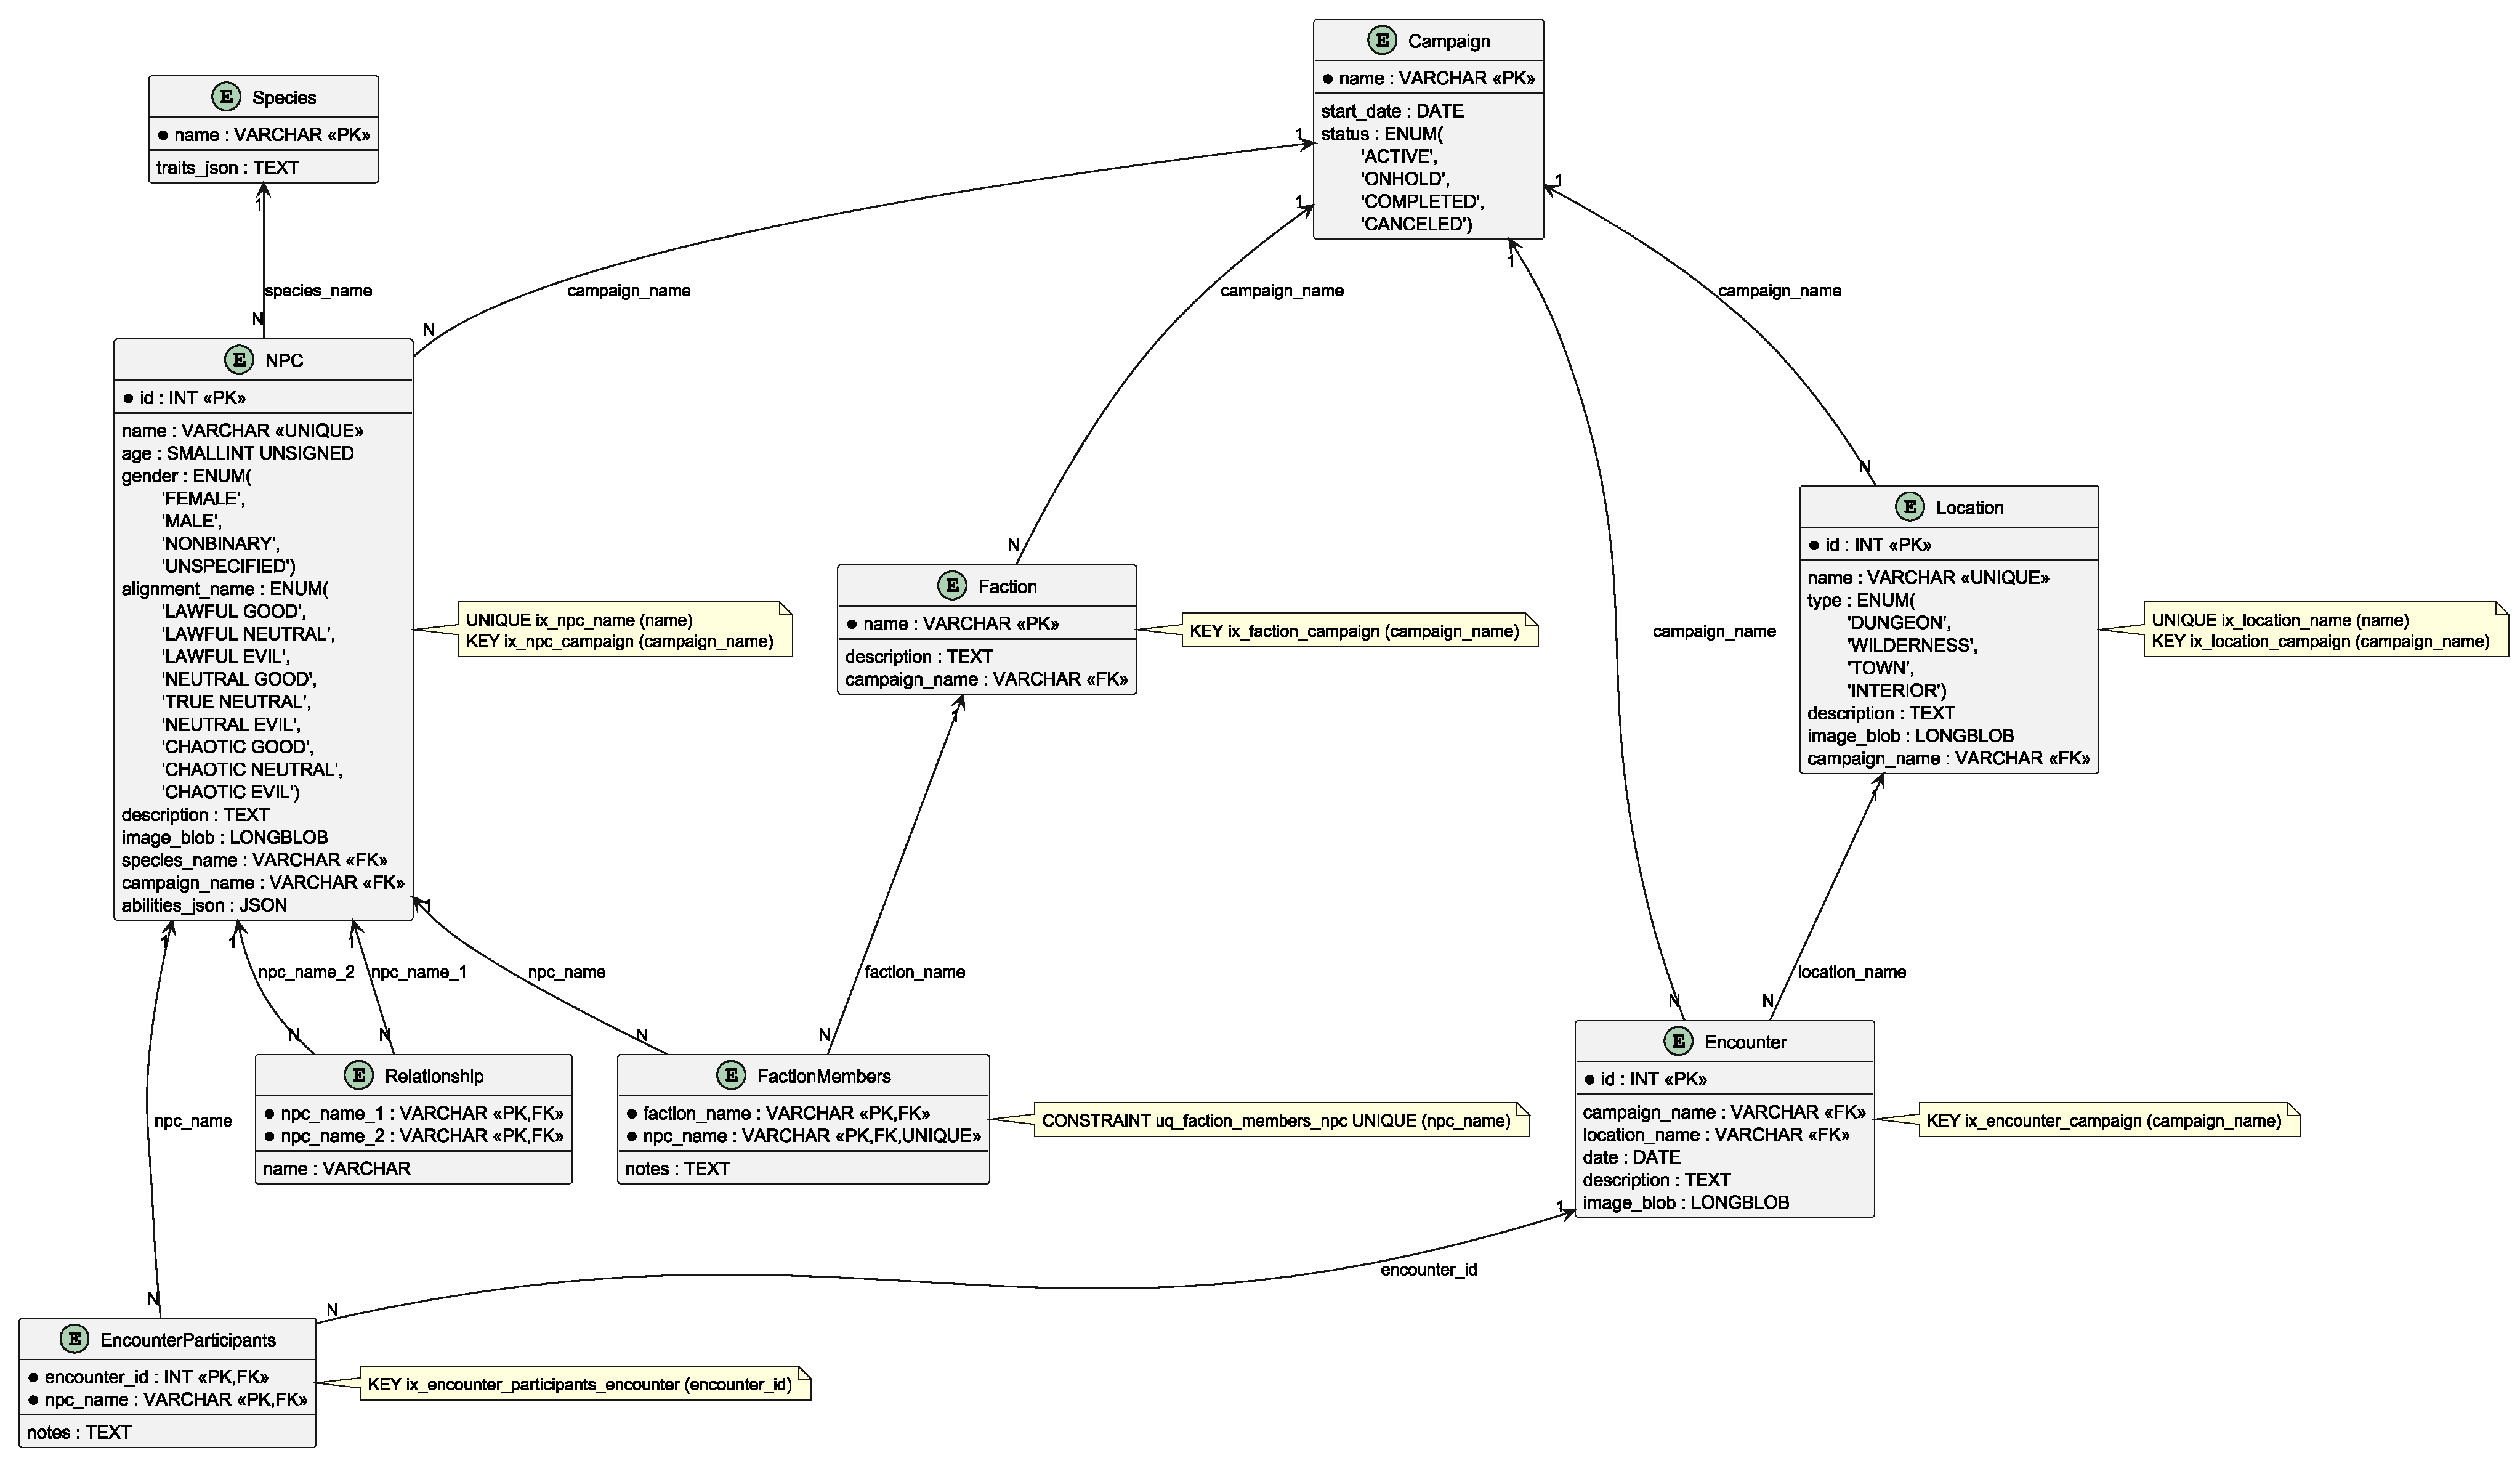
\includegraphics[width=0.99\textwidth]{ERD.eps}
\end{figure}

\section{Source of Data and Design Overview}
The project will be a python program utilizing the \keyword{customtkinter} library to create a \keyword{GUI}. It will follow best practices when it comes to development such as having test code using \keyword{pytest} and will be fully typed and will use both the realtime typechecking library \keyword{beartype} as well as the static type checker \keyword{mypy}. It will follow PEP-8 code conventions and will use the \keyword{ruff} linter to confirm it follows it. It will be an installable package using \keyword{hatch-build} and pyproject.toml.  It will have menus and forms to facilitate the various operations listed in the Core Features. I will provide a sample data set that will be loaded on initial opening of the program from csv files. This example data will show off the various capabilities of the program as well as provide examples of its use.

\end{document}